% Sample file on how to use subfiles.
\documentclass[ExampleMasters.tex]{subfiles}

\begin{document}

	\chapter{Evolutionary Algorithms for Optimisation}
	The problem of finding the optimum value of a non-convex, non-linear function is often solved by the use of an evolutionary algorithm. In specific, evolutionary algorithms excel at avoiding local optimae and in converging to the global optimum point sought. Commonly used techniques include genetic algorithms and particle swarm techniques among several others. Evolutionary algorithms are often compared n the basis of speed of convergence, utlisation to a wide range of problems and consistency in repeated runs of the algorithm. The cornerstone of the genetic algorithm in particular is the effective transmission of \textit{individual} information that contributes to optimum objective function performance.\\

	The challenge in the use of such algorithms lies in constructing the problem in a manner amenable to solution using the desired optimisation algorithm. The research in this thesis employs a standard genetic algorithm with a custom-defined genotype.\\

	\section{Elements of a standard Genetic Algorithm}
		The genetic algorithm draws inspiration from evolutionary processes seen in nature. Several randomly generated individuals are allowed to \textit{mate} and share genetic data and efficient \textit{stronger} individuals tend to be selected for such information transfers more often than \textit{weaker} individuals with characteristics that drive the objective function lower. Selected individuals mate and exchange genetic information producing offspring with strong genetic makeup and characteristics that replace the existing population. Occasional probabilistic genetic mutations help in discovering potentially \textit{strong} genome sequences that may accelerate the evolution of the species. While variations in any or all of these processes alter the efficacy of the algorithm, the prevalence of \textit{stronger} individuals over \textit{weaker} ones drives the evolution over several pre-defined number of generations.\\

		\subsection{Objective Function}
			The purpose of the optimisation technique is to identify the global maximum or minimum of a desired objective function that is defined in one or several variables / parameters. Such a function is mathematically constructed and a range within which the function optimum is desired is defined. For example, the two-variable benchmark Goldstein-Price function is defined as:
			\begin{multline}
				f(x,y)=(1+(x+y+1)^2(19-14x+3x^2-14y+6xy+3y^2))\\
					(30+(2x-3y)^2(18-32x+12x^2+48y-36xy+27y^2))
			\end{multline}

			whose global minima lies at $x=0$ and $y=-1$ and $f(0,-1)=-3$. In this research, the objective function to be maximised is the combination productivity as described in Chapter 2.\\

		\subsection{Individual representation and creation}
			The variables of the above defined objective function may be represented as a genetic sequence in a manner that allows a variety of data points where the function is defined to be created. Each set of data points $(x,y)$ may be called an \textit{individual}. Such individuals are often \textit{encoded} in binary or real-number formats. For example, an individual \textit{chromosome} containing 10 bits, 5 consecutive bits representing each variable $x$ and $y$ may look like:

			$$ 0     0     1     0     0     1     1     1     0     1$$

			The bits representing the encoded individual are the genetic material that is exchanged upon mating. A pre-defined number of such individuals constituting a \textit{population} form the breeding ground for the evolutionary exercise leading to the optimal solution. The individual structure and encoding scheme may, of course, vary to suit the problem at hand. The population of individuals is created stochastically using a pseudo-random number generator engine that generate integers based on a uniform distribution.\\

		\subsection{Decoding, Evaluation and Selection}
			Created individuals are decoded based on pre-set rules and the function value represented by each individual in the population is evaluated. For example, the above shown individual may be decoded to $(x,y) = (-2.2258, 2.6129)$. The Goldstein Price function defined above is evaluated to a value of $0.1711$ at this data point and is thus assigned as the individual's \textit{fitness}. From this created population, 2 or more individuals are \textit{selected} probabilistically and either repetitively or uniquely. Selected individuals mate to produce \textit{offspring} that replace the \textit{parents} in the population. Tournament selection and Roulette-wheel selection are often employed as stochastic selection mechanisms where the \textit{fitter} individual is selected over the \textit{weaker} with a preset probability.\\
		\subsection{Crossover}
			Such selected individuals exchange different portions of their genetic makeup in a stochastic fashion based on a pre-defined crossover probability. For example, individuals such as the ones shown above may be split at a random bit location beyond which all bits are exchanged with the other selected individual or individuals.\\ 
		\subsection{Mutation}
			Mimicking natural mutation processes that create varieties in genetic makeup leading to new features, random bits may, with a mutation probability, be mutated to another value. This may occassionally produce very fit individuals that can accelerate the evolution of the generation.\\
		\subsection{Elitism}
			The fittest individual in each generation may be preserved at the end of the generation so as to ensure that the information producing the best function values in that generation are not lost leading to oscillating best individual fitnesses in successive generations.\\

		These processes repeat for a number of decided generations until all individuals converge to the \textit{Vitruvian} individual representing the global optima of the objective function chosen to be optimised. The algorithm flowchart is depicted in Figure \ref{GAFlowchart} \cite{Wahde}.\\

		\begin{figure}[ht!]
			\centering
			\includegraphics[width=0.4\linewidth]{figures/GeneticAlgorithm/GAFlowchart.png}
			\caption{Genetic Algorithm Description Flowchart \cite{Wahde}}
			\label{GAFlowchart}
		\end{figure}

	\section{The Optimisation Problem}
		The previous chapter discusses how vehicle productivity is affected by the vehicle propulsion configuration. The problem at hand can thus be stated in words as\\
		
		\centerline{''\textit{Find} the vehicle combination that \textit{maximises} mission productivity over the first ownership duration"}. 

		Mathematically, the optimisation problem can be written as
		\begin{gather}
			\textit{Maximise}\  P\\
			where,\ P =\ f\Bigg(N_{Axle},\ P_{Axle},\ S_{Engine},\ S_{Buffer,i},\ S_{Motor,i}\Bigg)\\
			subject\ to,\ S_{Engine} \in {[Volvo\ D11,\ Volvo\ D13,\ Volvo\ D16]},\\
			S_{Buffer,i} \in {[5\ kWh,\ 50\ kWh,\ 91\ kWh]},\\
			S_{Motor,i} \in {[125\ kW\ \&\ 230\ Nm,\ 173\ kW\ \&\ 400\ Nm,\ 175\ kW\ \&\ 800\ Nm]},\\
			N_{Axle} \in {[1,8]},\ and\\
			P_{Axle} \in {[Axles\ [1,3]\ in\ Trailer\ 1,\ Axles\ [1,2]\ in\ Dolly\ ,\ Axles\ [1,3]\ in\ Trailer\ 2]}
		\end{gather}

		\subsection{Objective function}
			The objective function to be \textit{maximised} is the \textit{N-year mission productivity}. The mission productivity is as defined in Section 2.4. Hence, the vehicle combination that yields the \textit{highest mission productivity} is the output of the optimisation.

		\subsection{Design Variables}
			The mission productivity for a specific driving cycle and payload depends on the vehicle configuration. The base configuration is the standard A-Double with a 3-axle tractor, 3-axle semitrailer, 2-axle dolly and 3-axle semitrailer in order. The main design variables chosen in this problem are:

			\begin{itemize}
				\item \textbf{Axle Propulsion Configuration} - Additional electric propulsion may be added on one or more of the trailer axles.
				\item \textbf{Engine Size} - The size of the conventional powertrain in the tractor unit can be varied.
				\item \textbf{Buffer Size} - Trailing Units that contain one or more propelled axles are assigned an electric buffer / battery. The sizes of the electric buffers on different trailing units may be different.
				\item \textbf{Motor Size} - Each propelled axle in the trailing units may be powered by an electric motor of varying power and torque rating. All motors in a trailing unit with more than one propelled axle draw power from a \textit{single} buffer in the unit.
			\end{itemize}

			\begin{table}[ht]
				\caption{Design Variables - Ranges}
				\centering
				\begin{tabular}{c c c}
				\hline\hline
				Design Variable & Range & Range Size \\
				\hline
				Axle Propulsion Configuration & $\begin{matrix}
													3\ axles\ on\ Semi-trailer\ 1\\
													2\ axles\ on\ Dolly\\
													3\ axles\ on\ Semi-trailer\ 2\\
												\end{matrix}$ & $2^8$\\
				Engine Size & Volvo D11, D13 \& D16 & 3\\
				Buffer Size & 5 kWh, 50 kWh \& 91 kWh & 3\\
				Motor Size & 125 kW \& 230 Nm, 173 kW \& 400 Nm, 175 kW \& 800 Nm & 3 \\
				\hline
				\end{tabular}
				\label{table:designParameters}
			\end{table}

			Since the parameters that constitute vehicle productivity vary every 5 years, the optimal propulsion configuration can be re-evaluated once in 5 years. Also, since vehicle GCW in a given year drives revenues earned as well as operating costs, a unique optimal configuration can be arrived at for each GCW carried in a year.\\ 

			The problem thus stated, a custom evolutionary algorithm to identify these optimal configurations for
			\begin{itemize}
			\item Over the years 2015, 2020, 2025 and 2030
			\item For GCWs 50t, 60t, 70t and 80t
			\end{itemize}

		\subsection{Problem Constraints}
			There are no vehicle performance parameter constraints imposed on the problem. Instead, the \textit{depth of discharge of each electric buffer} is pre-determined as a function of longitudinal position as explained in Section 4.6.3.

	\section{Genotype description}
		
		The \textit{chromosome} structure or \textbf{genotype} is sought to completely contain all the above information for each unit in the combination. The \textit{categorical variable} or chromosome thus contains one set of information for each individual unit, totalling 4 sets of machine, buffer and axle propulsion information. The acronyms MG, BG and AG below stand for Machine Genes, Buffer Genes and Axle Genes respectively. Also, U followed by the number represents the unit number.\\

		\centerline{\framebox{MG (U1)}\framebox{BG (U1)}\framebox{AG (U1)}/\framebox{MG (U2)}\framebox{BG (U2)}\framebox{AG (U2)}/\\}
		\centerline{\framebox{MG (U3)}\framebox{BG (U3)}\framebox{AG (U3)}/\framebox{MG (U4)}\framebox{BG (U4)}\framebox{AG (U4)}\\}

		\subsection{Machine Genes}
			Three different machine sizes, both for the engine on the tractor and for electric motors for trailer axles, are considered. Hence, the machine \textit{gene set} consists of 3 bits, one of which can be high and the other two low for each unit.\\

			\centerline{\framebox{Machine Bit 1}\framebox{Machine Bit 2}\framebox{Machine Bit 3}}
			\vspace{0.1in}

			The position of the high bit represents the size of the machine. For example, the \textbf{machine gene set} on Unit 1\\

			\centerline{\framebox{0}\framebox{1}\framebox{0}}
			\vspace{0.1in}

			represents the mid-sized D13 engine while the machine gene set on Unit 3\\

			\centerline{\framebox{0}\framebox{0}\framebox{1}}
			\vspace{0.1in}

			represents the largest 175 kW, 800 Nm electric motor. This determines the size of the electric motor used to power all the Live axles in the specified Unit. Hence, variety of motor size within a Unit has been eliminated.\\

		\subsection{Buffer Genes}
			The same scheme as that for the \textbf{Machine Gene Set} is followed for the Buffer too, with the Gene Set containing 3 bits representing the three sizes of the electric buffer considered.\\

			\centerline{\framebox{Buffer Bit 1}\framebox{Buffer Bit 2}\framebox{Buffer Bit 3}}
			\vspace{0.1in}

			The buffer gene set for the Tractor is always set to three null bits as the size of the fuel tank on the tractor is constant.\\

		\subsection{Axle Genes}
			The number of bits in the \textbf{Axle Gene Set} are equal to the number of axles in the given unit. For example, the axle gene set of the first semitrailer contains 3 bits while that of the dolly contains 2 bits.\\

			\centerline{Tractor \& Semitrailers - \framebox{Axle Bit 1}\framebox{Axle Bit 2}\framebox{Axle Bit 3}}
			\vspace{0.1in}

			\centerline{Dolly - \framebox{Axle Bit 1}\framebox{Axle Bit 2}}
			\vspace{0.1in}

			A high bit indicates that the axle is \textit{live}, or Live, while a low bit indicates that the axle is \textit{dead} or Dead. For example,\\

			\centerline{\framebox{1}\framebox{0}\framebox{1}}
			\vspace{0.1in}

			indicates that Axle 1 and Axle 3 on the specified Unit are Live while Axle 2 remains Dead.\\

		A combination of these three gene sets provides complete propulsion information in a \textbf{Unit Gene Set} for a single Unit and a combination of these \textit{Unit Gene Sets} comprises the genotype. A sample chromosome is defined below and the vehicle configuration desribed for clarity.\\


			\centerline{\framebox{0}\framebox{0}\framebox{1} | \framebox{0}\framebox{0}\framebox{0} | \framebox{0}\framebox{1}\framebox{1} ||| \framebox{0}\framebox{0}\framebox{1} | \framebox{1}\framebox{0}\framebox{0} | \framebox{0}\framebox{0}\framebox{1} |||} 
			\centerline{| \framebox{0}\framebox{1}\framebox{0} | \framebox{1}\framebox{0}\framebox{0} | \framebox{0}\framebox{1} ||| \framebox{0} \framebox{0}\framebox{1} | \framebox{1}\framebox{0}\framebox{0} | \framebox{0}\framebox{0}\framebox{0}}

		\begin{table}[H]
			\caption{Sample Genome Decoding Scheme}
			\centering
			\begin{tabular}{c c c c c c c}
			\hline\hline
			Unit No. & Unit Type & Machine Size & Buffer Size & \multicolumn{3}{c}{Axle Configuration}\\ \cline{5-7}
			& & & & Axle 1 & Axle 2 & Axle 3\\
			\hline
			1 & Tractor & D16 Engine & 600 Litres & Dead & Live & Live \\
			2 & Semi-Trailer 1 & 173 kW, 800 Nm  Motor & 5 kW Battery & Dead & Dead & Live \\
			3 & Dolly & 125 kW, 400 Nm  Motor & 5 kW Battery & Dead & Live & - \\
			4 & Semi-Trailer 2 & - & None & Dead & Dead & Dead \\
			\hline
			\end{tabular}
			\label{table:genomeDecoding}
		\end{table}

		It can be noted above in Table \ref{table:genomeDecoding} that no buffer is created on a given Unit when all its axles remain Dead. The buffer and motor bits, though present, therefore remain insignificant. The above sample vehicle combination is pictorially represented as below in Figure \ref{genomeDecoding}.\\

		\begin{figure}[H]
			\centering
			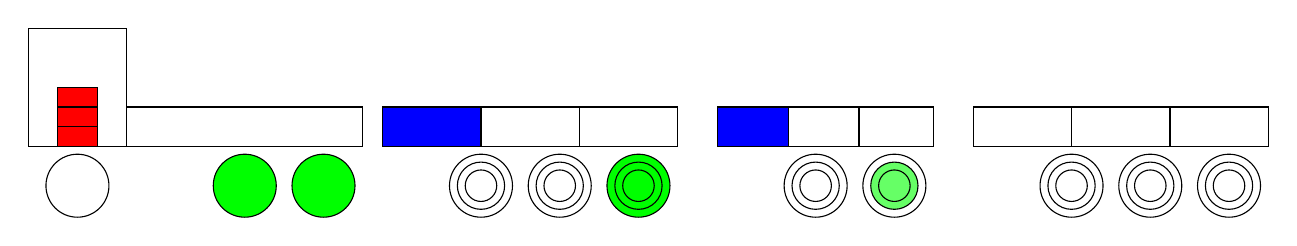
\begin{tikzpicture}[ scale=0.5]
				% Tractor
				\draw (7.5,2) rectangle (10,5);
				\draw[fill=red] (8.25,2) rectangle (9.25,2.5);
				\draw[fill=red] (8.25,2.5) rectangle (9.25,3);
				\draw[fill=red] (8.25,3) rectangle (9.25,3.5);
				\draw (10,2) rectangle (16,3);
				\draw (8.75,1) circle (0.8);
				\draw[fill=green!100] (13,1) circle (0.8);
				\draw[fill=green!100] (15,1) circle (0.8);

				% Semi-trailer
				\draw[fill=blue] (16.5,2) rectangle (19,3);
				\draw (19,2) rectangle (21.5,3);
				\draw (21.5,2) rectangle (24,3);
				% \draw (17,0.5) rectangle (18,1);
				% \draw (17,1) rectangle (18,1.5);
				% \draw (17,1.5) rectangle (18,2);
				\draw (19,1) circle (0.8);
				\draw (19,1) circle (0.6);
				\draw (19,1) circle (0.4);
				\draw (21,1) circle (0.8);
				\draw (21,1) circle (0.6);
				\draw (21,1) circle (0.4);	
				\draw[fill=green!100] (23,1) circle (0.8);
				\draw (23,1) circle (0.6);
				\draw (23,1) circle (0.4);

				% Dolly
				\draw[fill=blue] (25,2) rectangle (26.8,3);
				\draw (26.8,2) rectangle (28.6,3);
				\draw (28.6,2) rectangle (30.5,3);
				% \draw (25.5,0.5) rectangle (26.5,1);
				% \draw (25.5,1) rectangle (26.5,1.5);
				% \draw (25.5,1.5) rectangle (26.5,2);
				\draw (27.5,1) circle (0.8);
				\draw (27.5,1) circle (0.6);
				\draw (27.5,1) circle (0.4);	
				\draw (29.5,1) circle (0.8);
				\draw[fill=green!60] (29.5,1) circle (0.6);
				\draw (29.5,1) circle (0.4);	

				% Semi-trailer
				\draw (31.5,2) rectangle (34,3);
				\draw (34,2) rectangle (36.5,3);
				\draw (36.5,2) rectangle (39,3);
				% \draw (32,0.5) rectangle (33,1);
				% \draw (32,1) rectangle (33,1.5);
				% \draw (32,1.5) rectangle (33,2);
				\draw (34,1) circle (0.8);
				\draw (34,1) circle (0.6);
				\draw (34,1) circle (0.4);
				\draw (36,1) circle (0.8);
				\draw (36,1) circle (0.6);
				\draw (36,1) circle (0.4);	
				\draw (38,1) circle (0.8);
				\draw (38,1) circle (0.6);
				\draw (38,1) circle (0.4);
			\end{tikzpicture}
			\caption{Sample Combination Chromosome Decoding}
			\label{genomeDecoding}
		\end{figure}

		\subsection{Guide to pictorial representation}
		The combination represented in Figure \ref{genomeDecoding} is the standard mode of representation that will be used in the rest of the thesis. A description of the same is provided below with respect to the design variables listed in Section 3.2.2. (See Table \ref{table:designParameters})\\

		\begin{itemize}
			\item \textbf{Axle Propulsion Configuration} - All \textbf{propelled axles} in the combination are shown in \textbf{green}. All non-propelled axles are unshaded.
			\item \textbf{Engine Size} - The \textit{three vertically stacked blocks} in the tractor unit represent the engine size. The three blocks indicate the three sizes of the engines considered. \textbf{One block shaded red implies the D11 engine, two blocks, the D13 engine and all blocks, the D16 engine.}
			\item \textbf{Buffer Size} - The \textit{three horizontal blocks} in each trailing unit's chassis represent the varying sizes of the buffer. \textbf{One block shaded blue implies the smallest buffer, two blocks, the medium sized buffer and all blocks, the largest buffer.}
			\item \textbf{Motor size} - The \textit{three concentric circles in each wheel} in the combination represent the three varying sizes of the motors possible. \textbf{Only the smallest circle shaded green implies the smallest motor, two of the inner circles shaded represents the medium sized buffer and the complete wheel shaded represents the largest buffer.}
		\end{itemize}


	\section{Crossover, Mutation and Fitness Evaluation}
		Gene mutation follows the same protocol as in normal binary mutations with the added restriction that mutations can result in only one kind of machine or buffer being valid for a single unit. Crossovers are programmed in manner such that individual \textit{Gene Sets} are considered as the equivalents of single bits. In this manner, the chromosome described in Section 3.3 can be said to contain 12 such bits, 3 for each Unit. A crossover point is stochastically determined and crossover initiate with a predefined probability.\\

		For example, with the two \textit{selected} individuals shown below, a crossover is initiated at \textbf{Gene Set number 5} and the resulting crossed over individuals shown below.\\ 

		Individual 1:\\

			\centerline{\framebox{0}\framebox{0}\framebox{1} | \framebox{0}\framebox{0}\framebox{0} | \framebox{0}\framebox{1}\framebox{1} ||| \framebox{0}\framebox{0}\framebox{1} | \framebox{1}\framebox{0}\framebox{0} | \framebox{0}\framebox{0}\framebox{1} |||} 
			\centerline{| \framebox{0}\framebox{1}\framebox{0} | \framebox{1}\framebox{0}\framebox{0} | \framebox{0}\framebox{1} ||| \framebox{0} \framebox{0}\framebox{1} | \framebox{1}\framebox{0}\framebox{0} | \framebox{0}\framebox{0}\framebox{0}}
			\vspace{0.1in}

		Individual 2:\\

			\centerline{\framebox{0}\framebox{1}\framebox{0} | \framebox{0}\framebox{0}\framebox{0} | \framebox{0}\framebox{1}\framebox{1} ||| \framebox{1}\framebox{0}\framebox{0} | \framebox{0}\framebox{1}\framebox{0} | \framebox{1}\framebox{0}\framebox{1} |||} 
			\centerline{| \framebox{0}\framebox{1}\framebox{0} | \framebox{1}\framebox{0}\framebox{0} | \framebox{1}\framebox{1} ||| \framebox{0} \framebox{0}\framebox{1} | \framebox{1}\framebox{0}\framebox{0} | \framebox{0}\framebox{1}\framebox{0}}
			\vspace{0.1in}

		Crossed Over Individual 1:\\

			\centerline{\framebox{0}\framebox{0}\framebox{1} | \framebox{0}\framebox{0}\framebox{0} | \framebox{0}\framebox{1}\framebox{1} ||| \framebox{0}\framebox{0}\framebox{1} | \framebox{1}\framebox{0}\framebox{0} | \framebox{1}\framebox{0}\framebox{1} |||} 
			\centerline{| \framebox{0}\framebox{1}\framebox{0} | \framebox{1}\framebox{0}\framebox{0} | \framebox{1}\framebox{1} ||| \framebox{0} \framebox{0}\framebox{1} | \framebox{1}\framebox{0}\framebox{0} | \framebox{0}\framebox{1}\framebox{0}}
			\vspace{0.1in}

		Crossed Over Individual 2:\\

			\centerline{\framebox{0}\framebox{1}\framebox{0} | \framebox{0}\framebox{0}\framebox{0} | \framebox{0}\framebox{1}\framebox{1} ||| \framebox{1}\framebox{0}\framebox{0} | \framebox{0}\framebox{1}\framebox{0} | \framebox{0}\framebox{0}\framebox{1} |||} 
			\centerline{| \framebox{0}\framebox{1}\framebox{0} | \framebox{1}\framebox{0}\framebox{0} | \framebox{0}\framebox{1} ||| \framebox{0} \framebox{0}\framebox{1} | \framebox{1}\framebox{0}\framebox{0} | \framebox{0}\framebox{0}\framebox{0}}
			\vspace{0.1in}

		Individuals are parsed to create a vehicle model based on the architecture described in Chapter 4. The created vehicle model executes the mission based on input mission data to generate fuel and charge consumption, mission time and other mission outputs that are used to calculate the productivity of the combination created. This productivity is assigned as the individual's fitness measure.\\

	\section{Algorithm parameter settings}
		A population consisting of 30 individuals was randomly generated. Tournament selection was performed with a tournament size of 2 individuals and the tournament selection parameter was 0.75. The crossover probability was fixed 0.7 and the mutation probability was fixed at 0.05. The number of generations chosen was 100.\\

\end{document}